\subsection{Схема-1: Простой узел - кровавые узлы}
В узлах этой группы конец образует одну петлю, а затем пересекается сам с собой нечётное число раз.
Чётное число получить невозможно - конец не уйдёт в петлю.

Иначе его можно описать как калышку, в которую один или более раз пропущен ходовой конец.

\graphicspath{{\currentpath}}

\paragraph{Простой узел} образуется, если пробить колышку ходовым концом один раз.

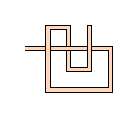
\includegraphics[scale=2]{images/double-simple-1-1.eps}
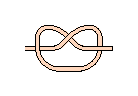
\includegraphics[scale=2]{images/simple.eps}

Вот так он выглядит сверху

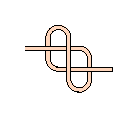
\includegraphics[scale=2]{images/simple-v2.eps}

\paragraph{Кровавый узел} образуется если к простому узлу добавить шлагов вокруг петли.

один шлаг

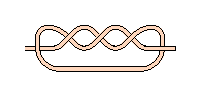
\includegraphics[scale=2]{images/blood-1.eps}

два шлага

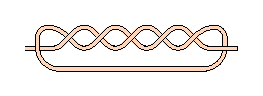
\includegraphics[scale=2]{images/blood-2.eps}

Второй вид узла

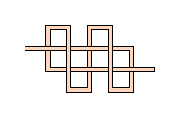
\includegraphics[scale=2]{images/blood-1-v2.eps}


\subsection{Схема-2: Удвоенный простой узел}

Если сложить вместе две калышки и пробить обе получится удвоенный простой узел


\includegraphics[scale=2]{images/double-simple-2-2.eps}

На скользкой верёвке с некоторым трудом можно завязать утроенный.

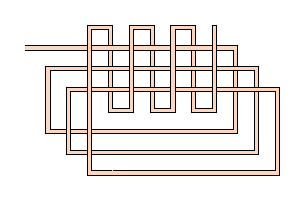
\includegraphics[scale=2]{images/double-simple-3-3.eps}
